\documentclass[12pt,a4paper]{report}	
\usepackage[utf8]{inputenc}
\usepackage{textcomp}
\usepackage{amsmath}
\usepackage{amsfonts}
\usepackage{amssymb}
\usepackage{color}
\usepackage{graphicx}
\usepackage{lscape}						%Landscape enabled. Doh!
\usepackage{longtable}					%To set table as multi-page
\usepackage{anysize}					%To set margins below
\marginsize{2cm}{2cm}{1cm}{3cm} 		%left, right, top, bot margin
\usepackage{float}						%Control table float
\usepackage{epstopdf}

\setcounter{secnumdepth}{3} %To get nummerated \subsubsection{title}
\setcounter{tocdepth}{3}	%To get nummerated \subsubsection{title}

\begin{document}
\section{Timebox 3}
\subsection{Outline for this timebox}

\begin{enumerate}
\item Design PCB for the Voltage \& Current measurement circuit
\item Design circuit for motor drivers
\item Inspect Regulator block
\item Design PWM circuit

\item Implement logger
\item Implement Relay server
\end{enumerate}


\subsection{Development Plan}
Jacob will be in charge of the first 4 steps, designing the circuits and the PCB, and inspect the regulator, to see exactly what is needed.\\
Morten and Henrik will be developing the software for the logger, and Morten will also finish the development of the Relay Server. 

\subsection{Results}


\input{tb3morten}

%

\input{tb3henrik}

\subsubsection{Design PCB for the Voltage \& Current measurement circuit (Jacob)}


\begin{figure}[h!]
\hspace*{-3cm}
\centering
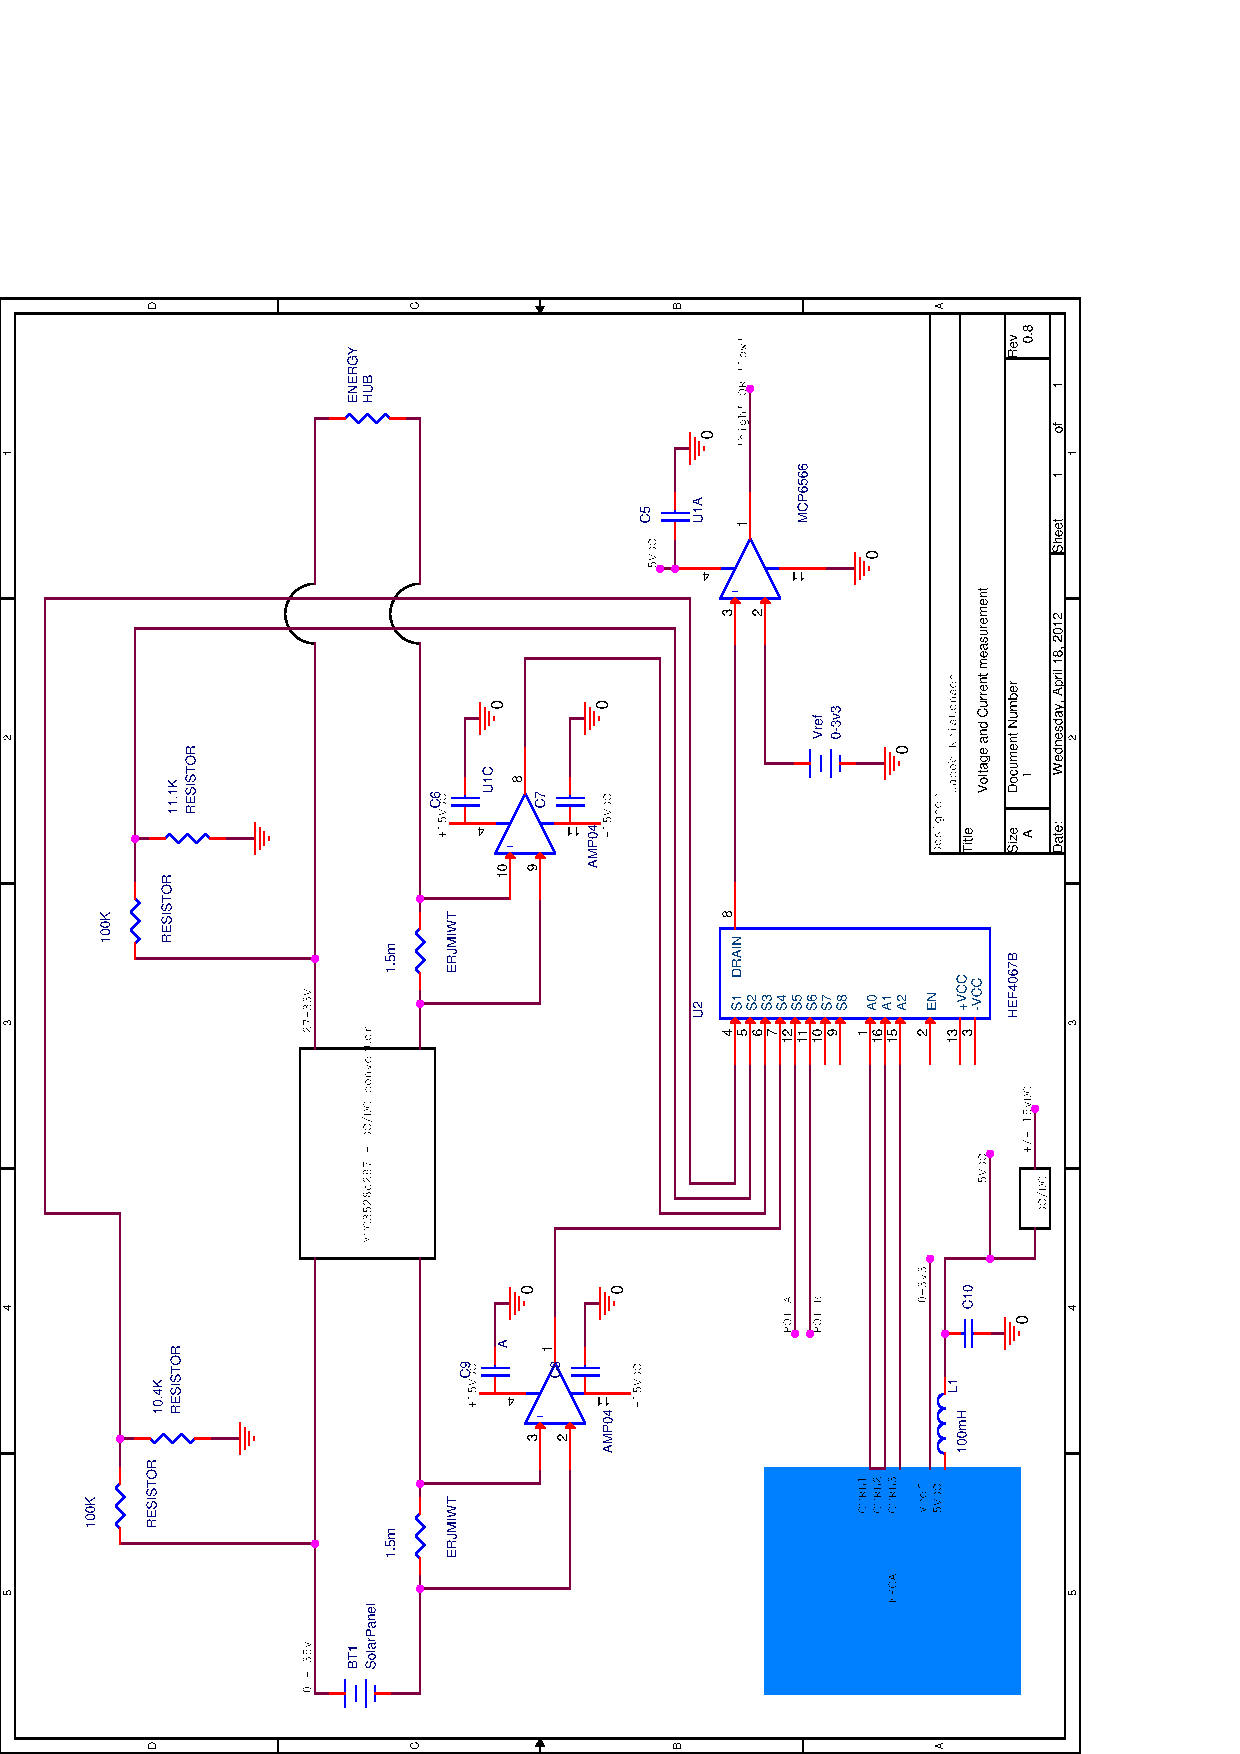
\includegraphics[width=13cm]{./img/SCHEMATIC1_VC_measurement}
\caption{Schematic - Voltage \& Current Measurement}
\label{fig:SCHEMATIC1_VC_measurement}
\end{figure}



\subsubsection{Design circuit for motor drivers (Jacob)}
\begin{figure}[h!]
\hspace*{-3cm}
\centering
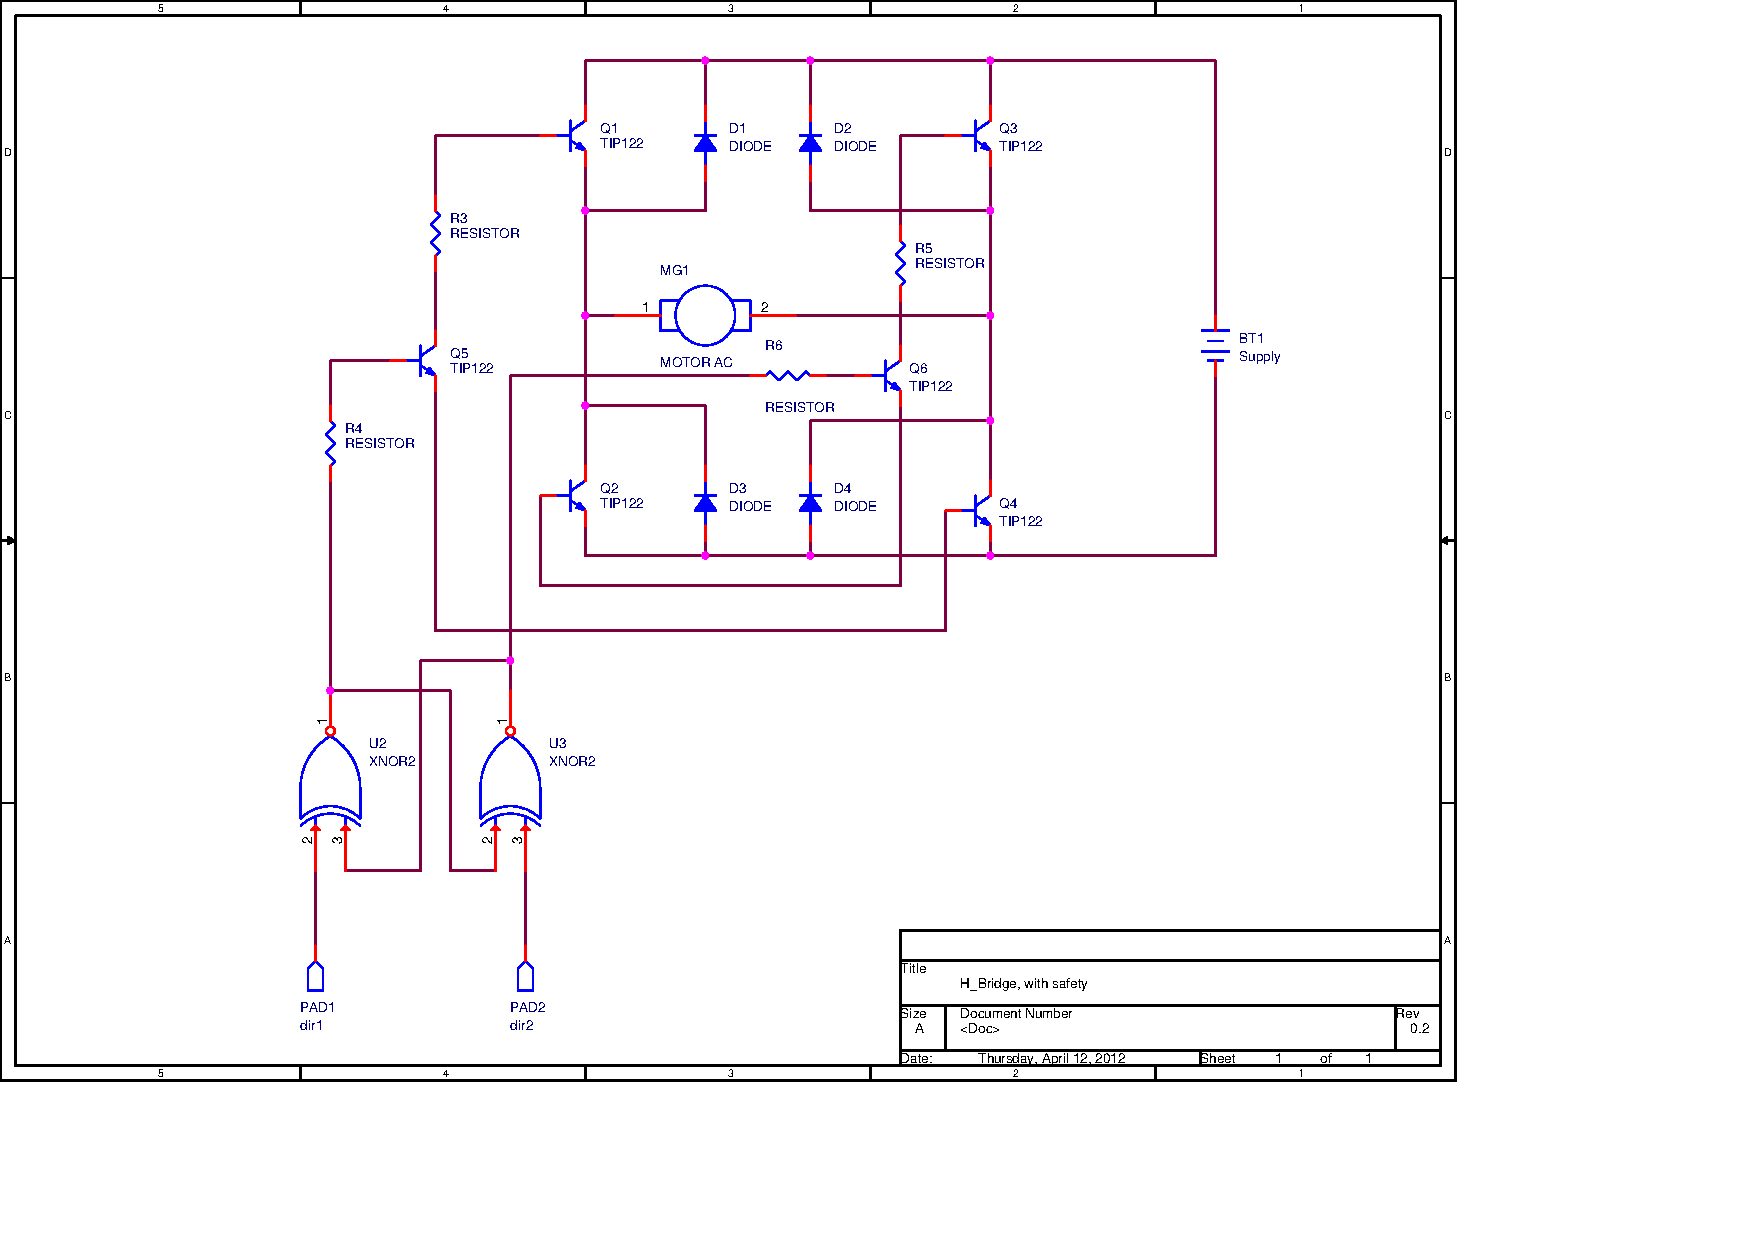
\includegraphics[width=13cm]{./img/SCHEMATIC1_H_Breidge}
\caption{Schematic - H-Bridge Motor control}
\label{fig:SCHEMATIC1_H_Breidge}
\end{figure}


\subsubsection{Inspect Regulator block (Jacob)}



\subsubsection{Design PWM circuit (Jacob)}
\begin{figure}[htbp]
\hspace*{-3cm}
\centering
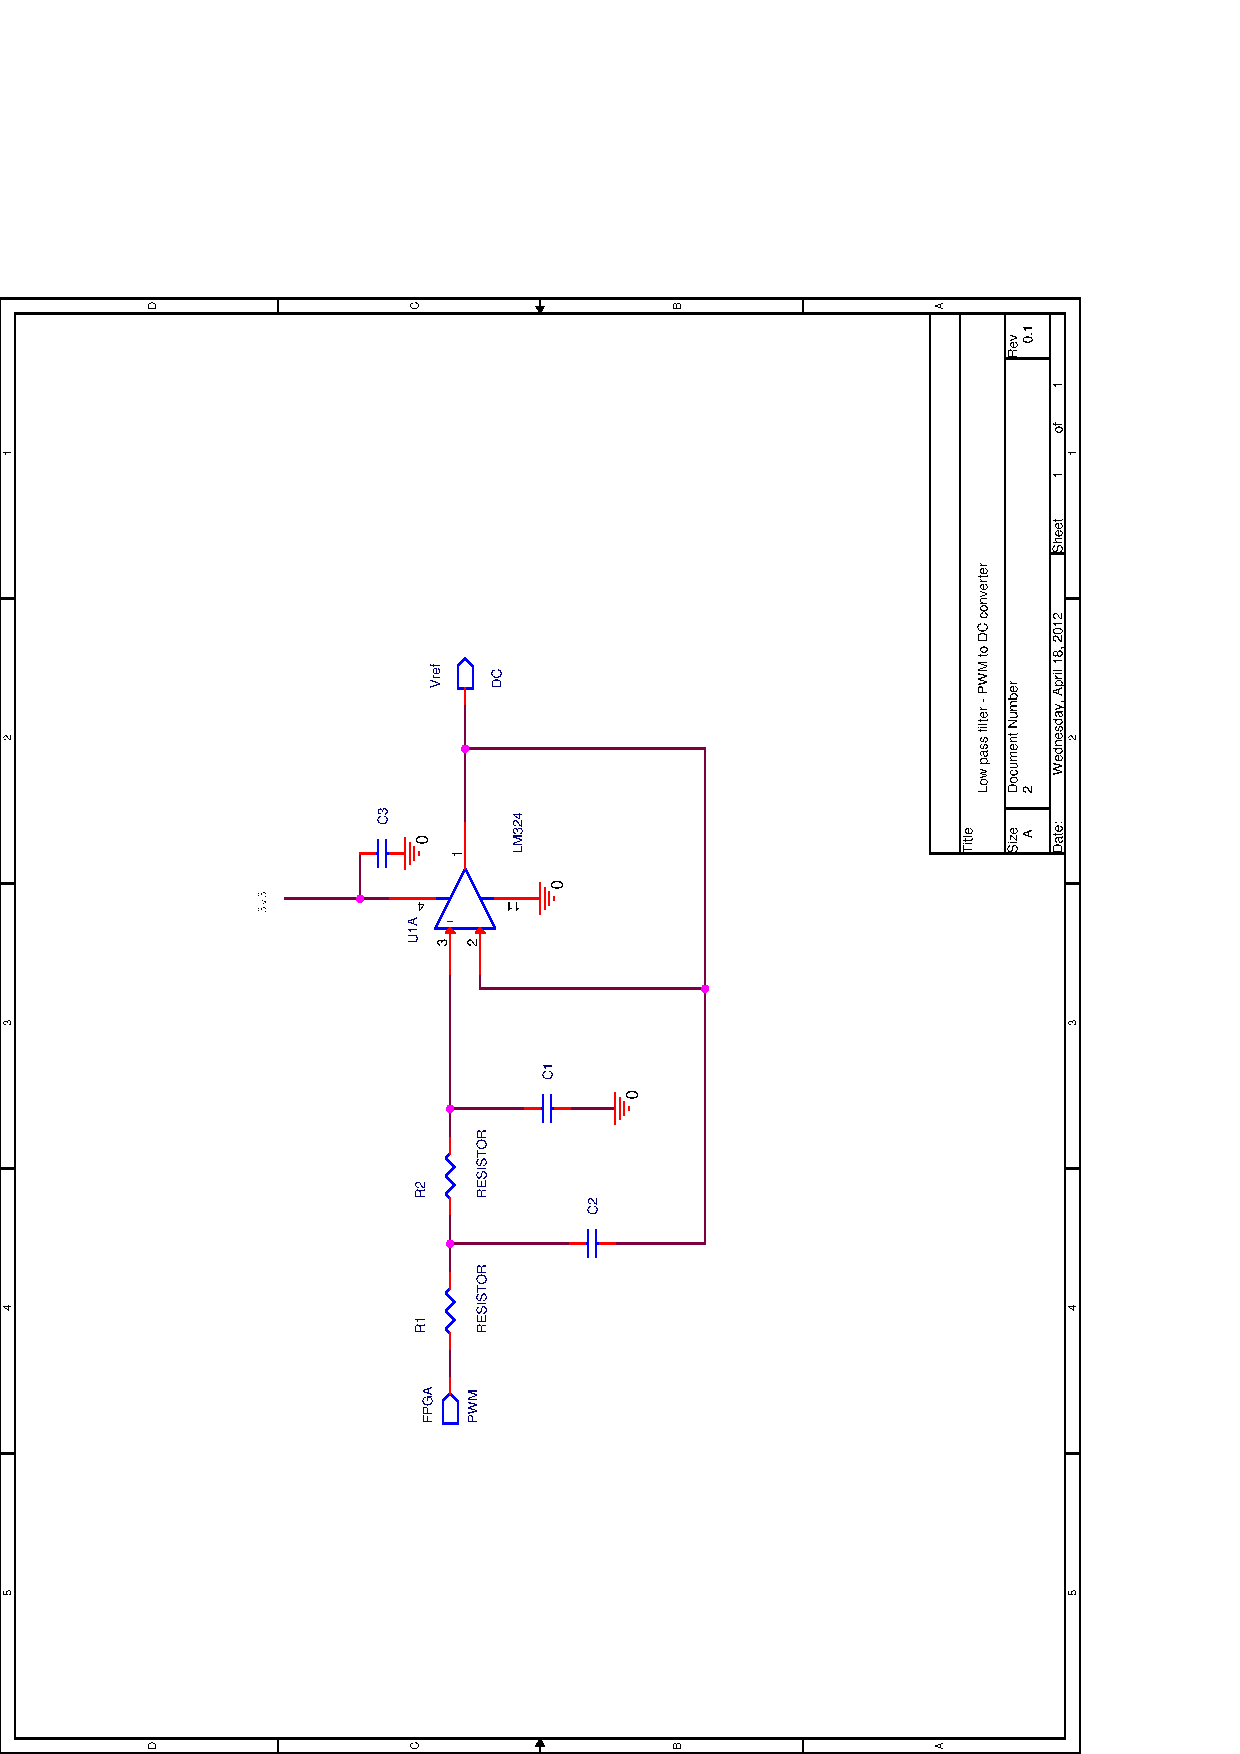
\includegraphics[width=13cm]{./img/SCHEMATIC1_PWM_DC}
\caption{Schematic - PWM to DC converter}
\label{fig:SCHEMATIC1_PWM_DC}
\end{figure}


\end{document}